\section{Zielsetzung}
In diesem Versuch sollen die grundsätzlichen Gesetzmäßigkeiten der Strahlenoptik, wie Reflexion und Transmission,
untersucht werden.

\section{Theorie}
\label{sec:Theorie}
Licht besteht aus elekromagntischer Strahlung und lässt sich durch verschiedene Zusammenhänge der Strahlenoptik beschreiben.
Das optische Spektrum des Lichts reicht von einer Wellenlänge von $\qty{100}{\nano\metre}$ bis $\qty{1}{\milli\metre}$, wobei
das menschliche Auge nur für Licht zwischen Wellenlängen von $\qty{380}{\nano\metre}$ bis $\qty{780}{\nano\metre}$ 
empflindlich ist.

\subsection{Reflexion und Transmission nach der Strahlenoptik}
In der Strahlenoptik wird die Ausbreitung von Lichtwellen über die Wellennormale beschrieben und eignet sich zur Beschreibung
von Reflexions- und Transmissionseffekten, nicht jedoch für manche andere Effekte, wie Interferenz oder Beugung. 

Trifft Licht auf eine Grenzfläche, so wird ein Teil reflektiert, wobei der Winkel des einfallenden Lichtstrahls dem Winkel
des ausfallenden Lichtstrahls gemäß
\begin{equation}
    \alpha_1 = \alpha_2 \label{eq:Reflexion}
\end{equation}
enspricht.
In verschiedenen Materialien breitet sich Licht mit unterschiedlichen Geschwindigkeiten aus. Aus diesem Grund verändert sich
der Weg des Lichts um einen Brechunswinkel. Mit materialabhängigen Brechungsindices $n$ ergibt sich für die Transmission
von Licht in ein anderes Medium die Relation
\begin{equation}
    n_1\sin\alpha = n_2\sin\beta. \label{eq:Brechung}
\end{equation}
Die Ausbreitungsgeschwindigkeit verändert sich zu
\begin{equation}
    v = \frac{c}{n}. \label{eq:Ausbreitungsgeschwindigkeit}
\end{equation}
In aller Regel wird ein Teil des auf eine Grenzfläche treffenden Lichts relektiert und der restliche Teil transmittert durch die 
Grenzfläche in das andere Medium. Es ergibt sich, dass der transmittert Teil $T$ und der reflektierte Teil $R$ zusammen genau
dem einfallenden Teil entsprechen müssen, also gilt $T + R = 1$.
In \autoref{fig:Brechungstypen} sind die beschriebenen Sachverhalte nochmals graphisch veranschaulicht.
\begin{figure}[H]
    \begin{subfigure}{0.31\textwidth}
      \centering
      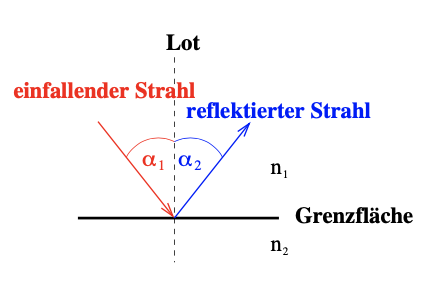
\includegraphics[height=5cm]{content/pics/Reflexion.png}
      \caption{Reflexion.}
    \end{subfigure}
    \hfill
    \begin{subfigure}{0.31\textwidth}
      \centering
      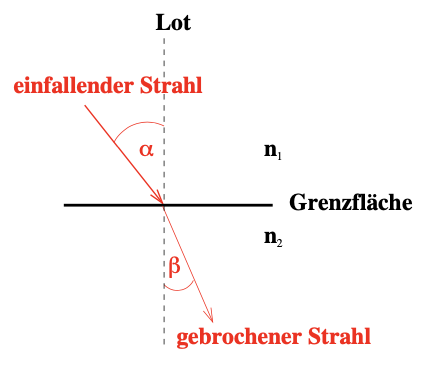
\includegraphics[height=5cm]{content/pics/Brechung.png}
      \caption{Transmission.}
    \end{subfigure}
    \begin{subfigure}{0.31\textwidth}
        \centering
        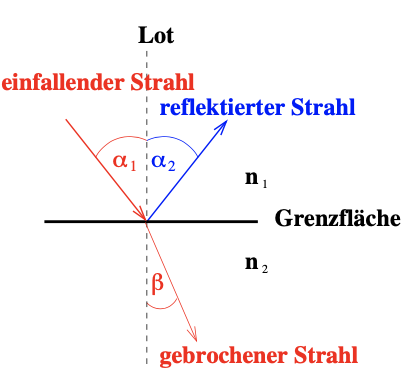
\includegraphics[height=5cm]{content/pics/Reflexion_Brechung.png}
        \caption{Reflexion und Transmission.}
      \end{subfigure}
    \caption{Skizzierung der Reflexion und Transmission von Licht \cite{v400}.}
    \label{fig:Brechungstypen}
  \end{figure}
Die Brechung von Licht hat zur Folge, dass Lichtstrahlen unter einem Strahlenversatz aus einer planparallelen Platte wieder 
austreten. Dies ist in \autoref{fig:Planparallel} dargestellt.
\begin{figure}[H]
    \centering
    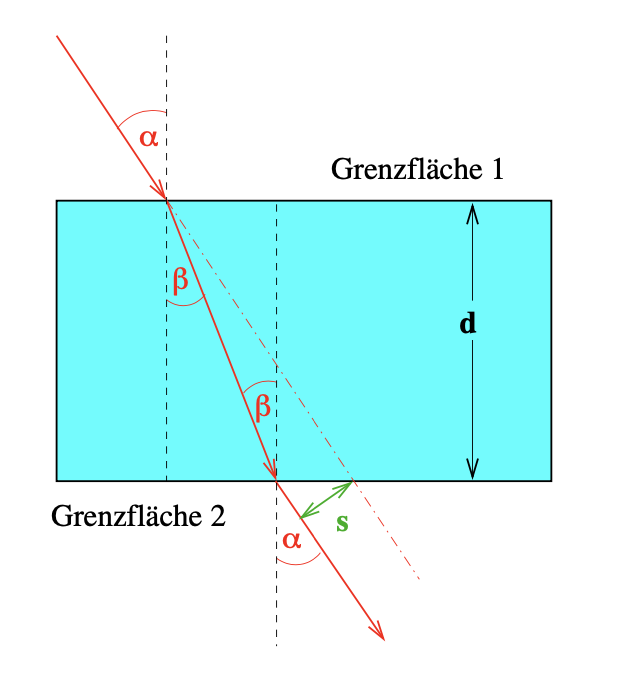
\includegraphics[height=7.5cm]{content/pics/Planparallel.png}
    \caption{Strahlenverlauf in einer planparallelen Platte \cite{v400}.}
    \label{fig:Planparallel}
\end{figure}
Für den Strahlenversatz $s$ ergibt sich die Gleichung
\begin{equation}
    s = d \frac{\sin(\alpha-\beta)}{\cos\beta}. \label{eq:Strahlenversatz}
\end{equation}

Für ein Prisma entsteht ein ähnlicher Zusammenhang. Hier wird der Strahlenversatz durch einen Winkel $\delta$ beschrieben, der 
wie in \autoref{fig:Prisma} definiert ist.
\begin{figure}[H]
  \centering
  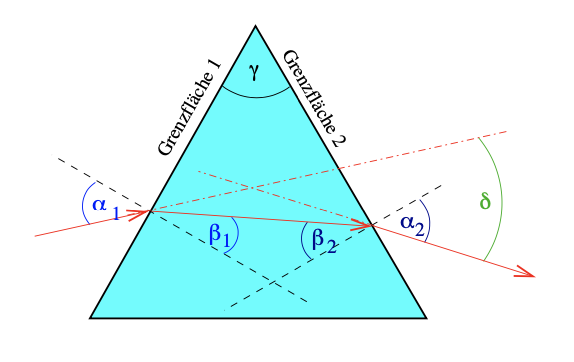
\includegraphics[height=5.5cm]{content/pics/Prisma.png}
  \caption{Strahlenverlauf in einem Prisma \cite{v400}.}
  \label{fig:Prisma}
\end{figure}
Für den Winkel $\delta$ folgt
\begin{equation}
  \delta = (\alpha_1+\alpha_2) - (\beta_1+\beta_2). \label{eq:Winkelbeziehung}
\end{equation}

\subsection{Beugung am Gitter nach der Wellenoptik}
Mithilfe der Wellenoptik lassen sich Effekte wie Interferenzbilder erklären. Dabei wird Licht als Welle angenommen und es gilt
demnach das Superpositionsprinzip, wonach sich Wellen überlagern können.
Ebenfalls relevant ist das Huygensche Prinzip, welches besagt, dass im Falle einer Brechung einer Welle jeder Punkt der Welle 
Ausgangspunkt einer neuen Elementarwelle mit selber Phase und Frequenz ist und die Einhüllende aller Elementarwellen die neue 
Wellenfront bildet.

Trifft eine Wellenfront auf ein Brechungsgitter lässt sich das auftretende Interferenzmuster mit eben diesen beiden Prinzipien
erklären und die durch konstruktive Interferenz auftretenden Intersitätsmaxima genügen dem Zusammenhang
\begin{equation}
    d\sin\alpha = k\lambda. \label{eq:Gitter}
\end{equation}
Hierbei bezeichnet $d$ die Gitterkonstante, also die Breite der Öffnung der einzelnen Gitterspalten. Der Winkel $\alpha$ wird
zwischen dem $k$-ten Intensitätsmaximum und dem Gitter gemessen und $k\lambda$ ist ein ganzzahliges Vielfaches der Wellenlänge
des einfallenden Lichts.
